
\chapter{INTRODUCTION}

\section{{\bf{Background}}}

The availability of enormous volumes of data in the healthcare industry in recent years has greatly increased the prospects for understanding and enhancing decision-making. A key tool for identifying patterns, trends, and correlations in large medical datasets is exploratory data analysis (EDA). To visualize these insights and support data-driven decision-making in the healthcare industry, interactive dashboard creation has also become crucial.\\
\noindent
The necessity to use EDA and dashboard generation to solve issues and enhance healthcare procedures is what spurred this project's inception. The sheer volume and complexity of medical data are often too much for traditional analysis tools to manage, making it difficult to draw useful conclusions.Data scientists and healthcare professionals can find hidden patterns, outliers, and correlations in the data by using EDA's systematic and exploratory methodology.\\
\noindent
Additionally, interactive dashboards that visualize these insights are a potent tool for better data communication and decision-making. Healthcare personnel may engage with data visualizations, personalize views, and receive insightful information quickly thanks to dashboards' straightforward and user-friendly interfaces. EDA and dashboard development have the power to transform healthcare procedures, maximize resource use, and improve patient care.


\section{{\bf{Objectives}}}
{The Objectives of this project were as follows
\begin{enumerate}
 \item Familiarity with data cleaning, feature extraction, and data conversion. 
 \item Describing the data using statistical method such as mean, median, standard deviation, correlation and so on. 
 \item Implementation of different plots in R to understand the data better. 
 \item Implementation of a dashboard.
 \item Understanding and explaining the trends and outliers in the data based on the domain.
\end{enumerate}
}

\section{\bf Significance}
Exploratory data analysis (EDA) and the development of interactive dashboards hold the potential to transform healthcare procedures, which is why this initiative is significant. This research intends to identify useful insights, such as correlations, trends, and risk factors that can significantly influence decision-making in the healthcare industry by conducting a thorough EDA on medical data. These insights can aid healthcare practitioners in maximizing resource allocation, enhancing overall health care plans, and improving patient outcomes. A user-friendly platform for visualizing and analyzing these insights will be provided by the creation of an interactive dashboard customized to the requirements of healthcare professionals, enabling users to make defensible decisions based on data-driven evidence.



\section{\bf Limitations}
The data used in this project is synthetic, meaning it has been artificially generated to simulate real-world medical data. Although synthetic data allows for controlled experiments and can provide valuable insights, it may not fully capture the complexity and nuances of actual patient data. The findings and conclusions drawn from the analysis should be interpreted with caution, considering the inherent differences between synthetic and real-world data. Efforts have been made to ensure the quality of synthetic dataset, but there is still a possibility of errors or limitations in the data generation process. The availability of computational resources and time constraints may also impact the scope and depth of the analysis. Despite these limitations, this project serves as an exploration of the potential benefits and challenges associated with synthetic medical data in the context of exploratory data analysis and dashboard creation. It provides insights into the effectiveness of these methodologies and offers considerations for future research utilizing real-world medical data.

\section{\bf Specifications}
-  Language: R (tidy-verse packages, dashboard packages).\\
-  IDE: Jupyter notebook and RStudio\\
-  Dashboard tool: flexboard package and \url{https://visual.is}\\
-  Data: Kaggle dataset\\

\begin{figure}[htpb]
\begin{center}
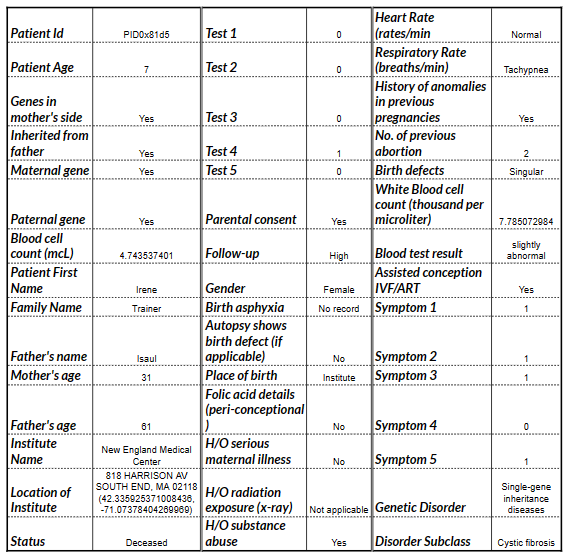
\includegraphics[height=10cm, width=12cm]{figures/sample.png}
\caption{Sample Data Of The Project}
\label{fig 1}
\end{center}
\end{figure}
